\documentclass[12pt,titlepage]{article}
\usepackage[margin=1.25in]{geometry}
\usepackage{graphicx,amsmath,minted}

%% Variables definition
\newcommand{\vSubject}{Database}
\newcommand{\vSubtitle}{Lesson 5}
\newcommand{\vName}{Dicha Zelianivan Arkana}
\newcommand{\vNIM}{2241720002}
\newcommand{\vClass}{1i}
\newcommand{\vDepartment}{Information Technology}
\newcommand{\vStudyProgram}{D4 Informatics Engineering}

%% [START] Tikz related stuff
\usepackage{tikz}
\usetikzlibrary{svg.path,calc,shapes.geometric,shapes.misc}
\tikzstyle{terminator} = [rectangle, draw, text centered, rounded corners = 1em, minimum height=2em]
\tikzstyle{preparation} = [chamfered rectangle, chamfered rectangle sep=0.75em, draw, text centered, minimum height = 2em]
\tikzstyle{process} = [rectangle, draw, text centered, minimum height=2em]
\tikzstyle{decision} = [diamond, aspect=2, draw, text centered, minimum height=2em]
\tikzstyle{data}=[trapezium, draw, text centered, trapezium left angle=60, trapezium right angle=120, minimum height=2em]
\tikzstyle{connector} = [line width=0.25mm,->]
%% [END] Tikz related stuff

%% [START] Fancy header related stuff
\usepackage{fancyhdr}
\pagestyle{fancy}
\setlength{\headheight}{15pt} % compensate fancyhdr style
\fancyhead{}
\fancyfoot{}
\fancyfoot[L]{\thepage}
\fancyfoot[R]{\textit{\vSubject - \vSubtitle}}
\renewcommand{\footrulewidth}{0.4pt}% default is 0pt, overline for footer
%% [END] Fancy header related stuff

%% [START] Custom tabular command related stuff
\usepackage{tabularx}
\newcommand{\details}[2]{
    #1 & #2  \\
}
%% [END] Custom tabular command related stuff

%% [START] Figure related stuff
\newcommand{\image}[3][1]{
    \begin{figure}[h]
        \centering
        \includegraphics[#1]{#2}
        \caption{#3}
        \label{#3}
    \end{figure}
}
%% [END] Figure related stuff

\begin{document}
\begin{titlepage}
    \centering
    \vfill
    {\bfseries\LARGE
        \vSubject\\
        \vskip0.25cm
        \vSubtitle
    }
    \vfill
    
\includegraphics[width=6cm]{images/polinema-logo.png}
    \vfill
    {
        \textbf{Name}\\
        \vName\\
        \vskip0.5cm
        \textbf{NIM}\\
        \vNIM\\
        \vskip0.5cm
        \textbf{Class}\\
        \vClass\\
        \vskip0.5cm
        \textbf{Department}\\
        \vDepartment\\
        \vskip0.5cm
        \textbf{Study Program}\\
        \vStudyProgram
    }
\end{titlepage}

\section{Database Diagram}
\begin{figure}[h]
    \centering
    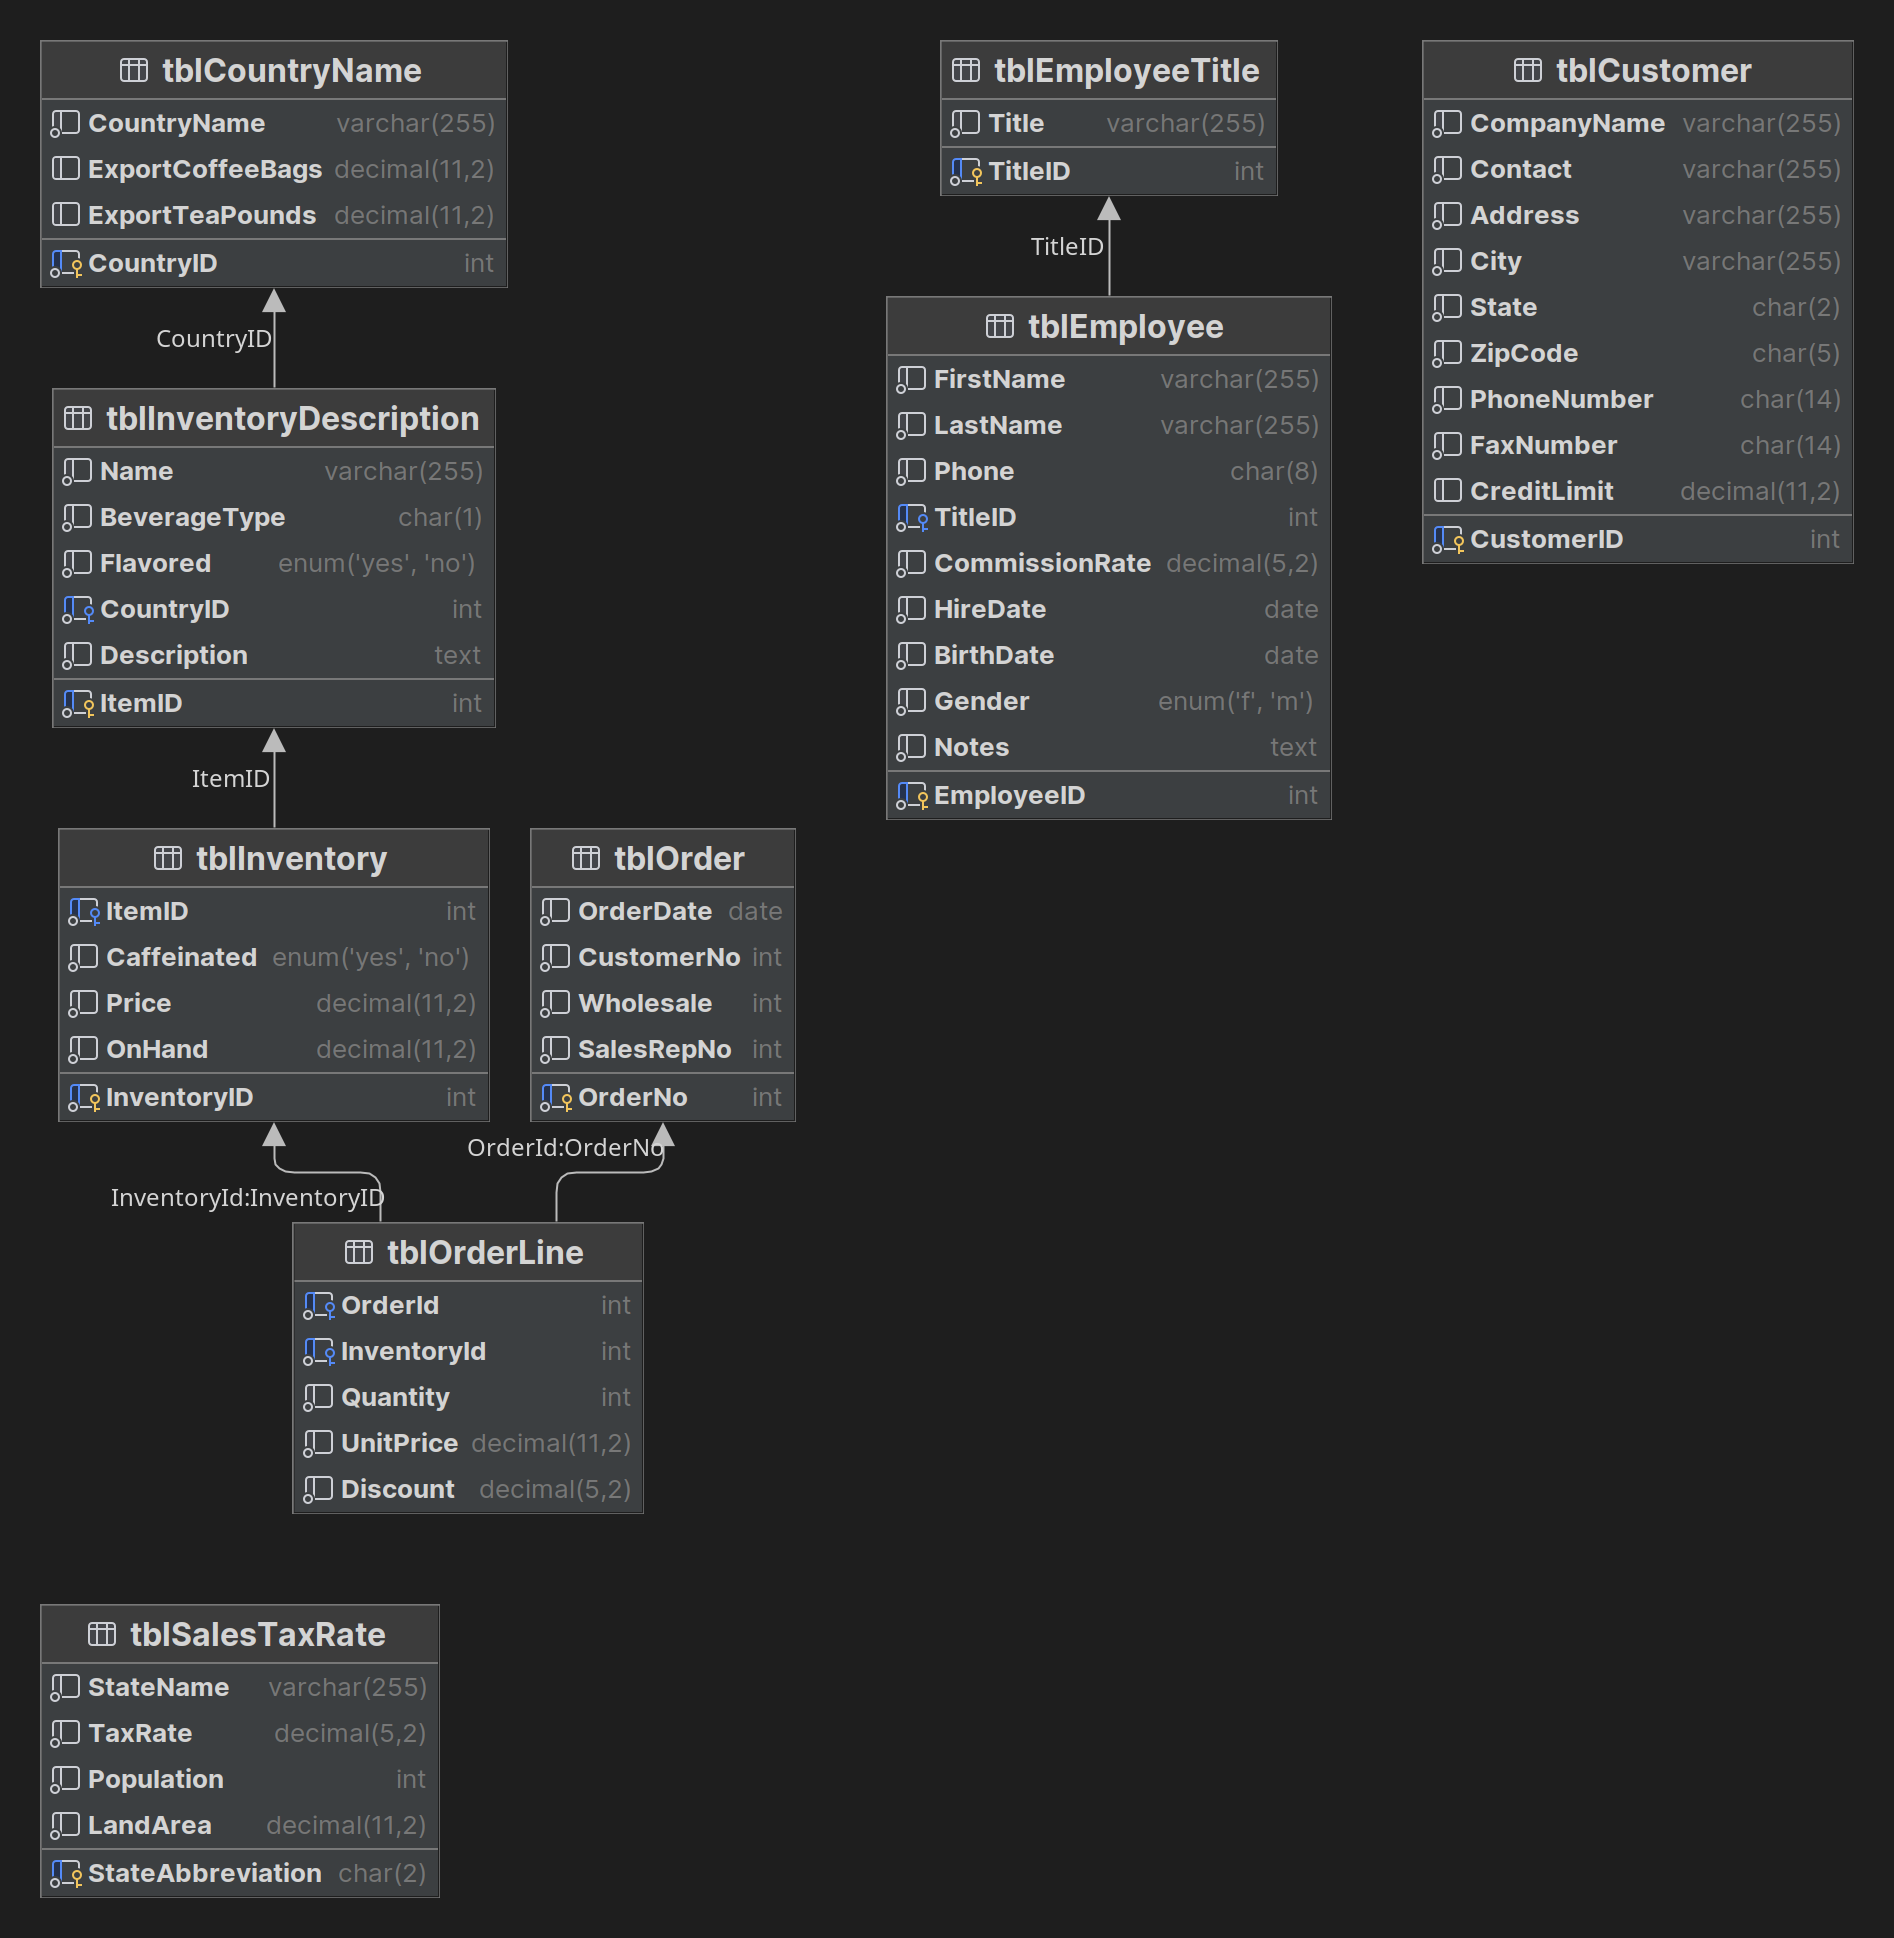
\includegraphics[width=\textwidth]{./images/diagram.png}
\end{figure}

\pagebreak

\section{Table Result}
\begin{itemize}
    \item {
        \textbf{tblCountryName}
        \begin{figure}[h]
            \centering
            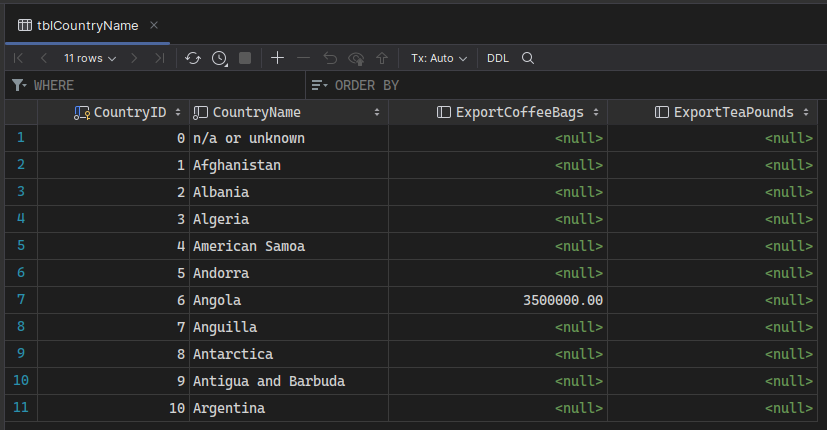
\includegraphics[width=.7\textwidth]{./images/tblCountryName.png}
        \end{figure}
    }
    \item {
        \textbf{tblCustomer}
        \begin{figure}[h]
            \centering
            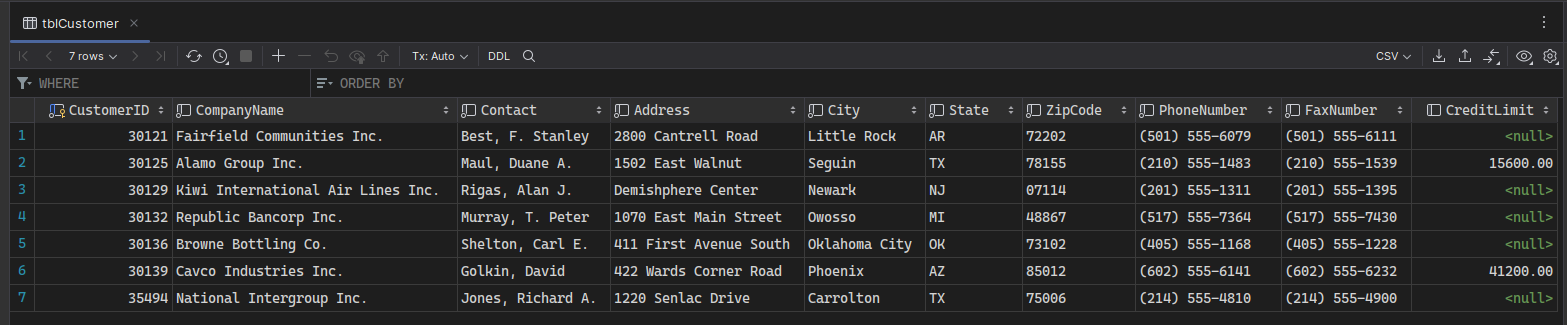
\includegraphics[width=.7\textwidth]{./images/tblCustomer.png}
        \end{figure}
    }
    \item {
        \textbf{tblEmployee}
        \begin{figure}[h]
            \centering
            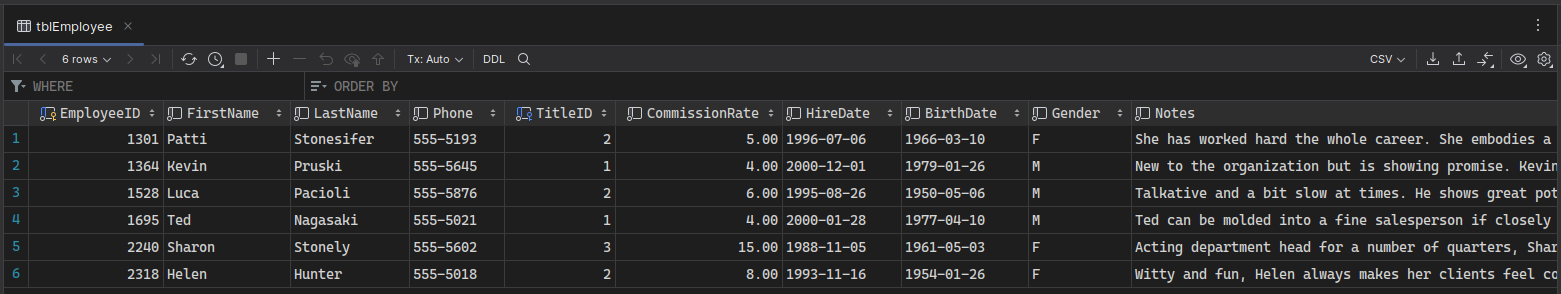
\includegraphics[width=.7\textwidth]{./images/tblEmployee.png}
        \end{figure}
    }
    \pagebreak
    \item {
        \textbf{tblEmployeeTitle}
        \begin{figure}[h]
            \centering
            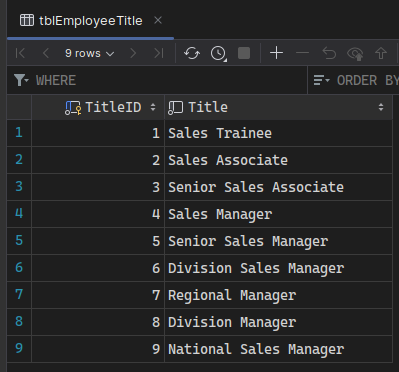
\includegraphics[width=.7\textwidth]{./images/tblEmployeeTitle.png}
        \end{figure}
    }
    \item {
        \textbf{tblInventory}
        \begin{figure}[h]
            \centering
            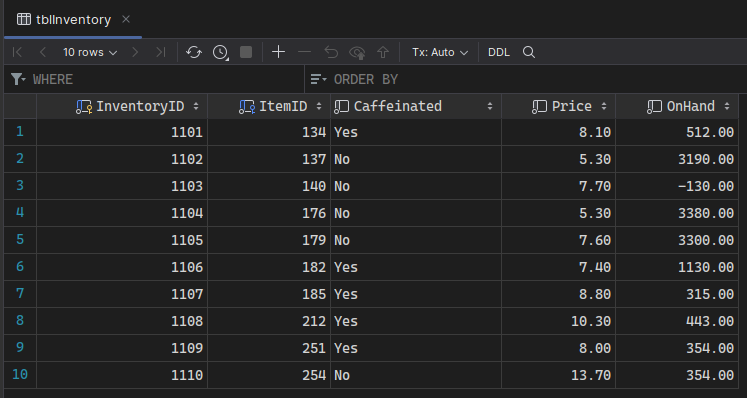
\includegraphics[width=.7\textwidth]{./images/tblInventory.png}
        \end{figure}
    }
    \pagebreak
    \item {
        \textbf{tblInventoryDescription}
        \begin{figure}[h]
            \centering
            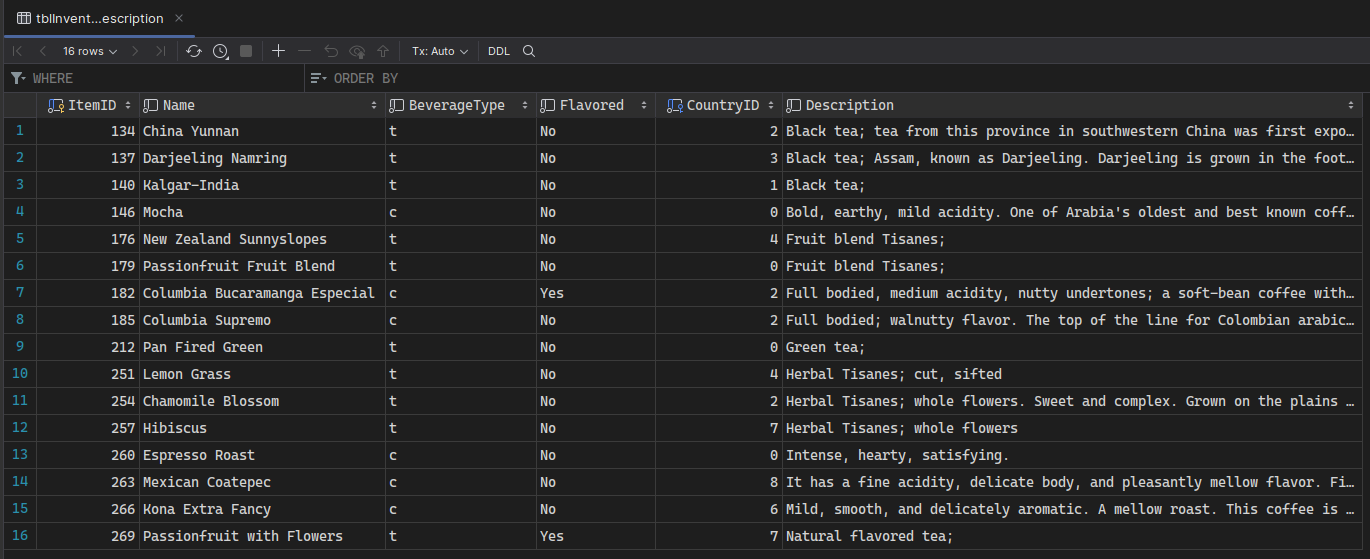
\includegraphics[width=.7\textwidth]{./images/tblInventoryDescription.png}
        \end{figure}
    }
    \item {
        \textbf{tblOrder}
        \begin{figure}[h]
            \centering
            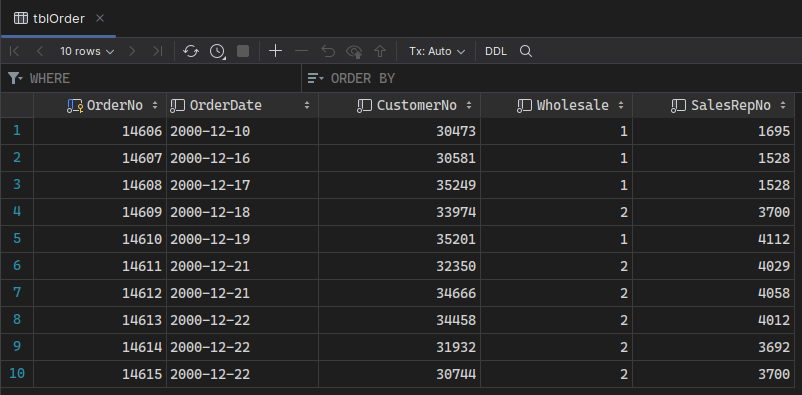
\includegraphics[width=.7\textwidth]{./images/tblOrder.png}
        \end{figure}
    }
    \pagebreak
    \item {
        \textbf{tblOrderLine}
        \begin{figure}[h]
            \centering
            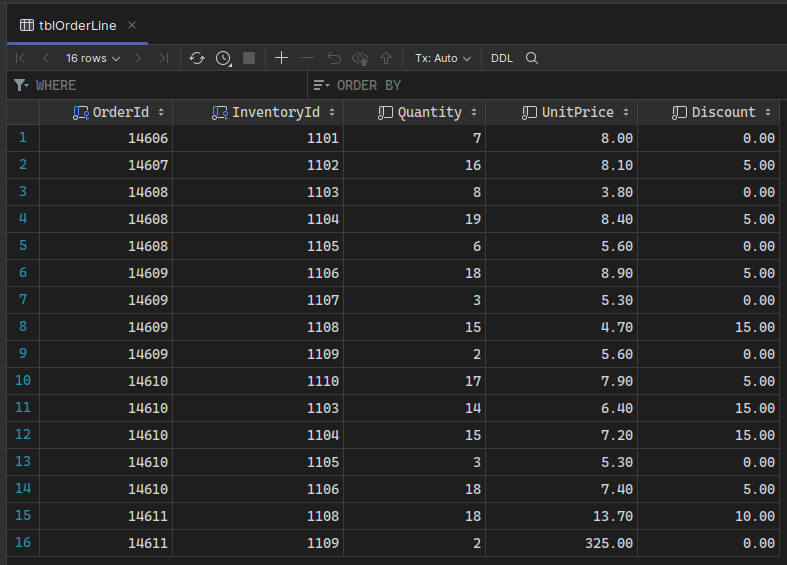
\includegraphics[width=.7\textwidth]{./images/tblOrderLine.png}
        \end{figure}
    }
    \item {
        \textbf{tblSalesTaxRate}
        \begin{figure}[h]
            \centering
            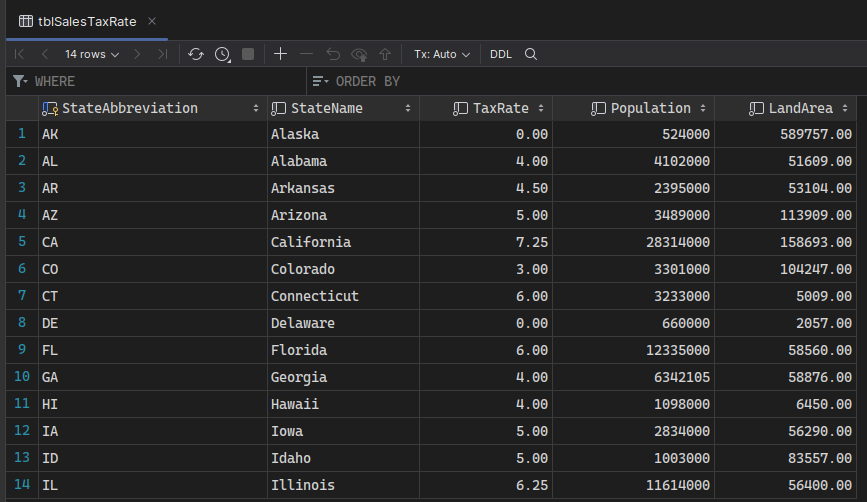
\includegraphics[width=.7\textwidth]{./images/tblSalesTaxRate.png}
        \end{figure}
    }
\end{itemize}

\pagebreak

\section{DDL - Data Definition Language}
\subsection{Creating Database}
\begin{minted}[autogobble,fontsize=\small]{sql}
    CREATE TABLE tblCountryName
    (
        CountryID        INT            NOT NULL PRIMARY KEY,
        CountryName      VARCHAR(255)   NOT NULL,
        ExportCoffeeBags DECIMAL(11, 2) NULL,
        ExportTeaPounds  DECIMAL(11, 2) NULL
    );
    
    CREATE TABLE tblInventory
    (
        InventoryID INT                NOT NULL PRIMARY KEY AUTO_INCREMENT,
        ItemID      INT                NOT NULL,
        Caffeinated ENUM ('Yes', 'No') NOT NULL,
        Price       DECIMAL(11, 2)     NOT NULL,
        OnHand      DECIMAL(11, 2)     NOT NULL
    );
    
    CREATE TABLE tblOrder
    (
        OrderNo    INT  NOT NULL PRIMARY KEY AUTO_INCREMENT,
        OrderDate  DATE NOT NULL,
        CustomerNo INT  NOT NULL,
        Wholesale  INT  NOT NULL,
        SalesRepNo INT  NOT NULL
    );
    
    CREATE TABLE tblOrderLine
    (
        OrderId     INT            NOT NULL,
        InventoryId INT            NOT NULL,
        Quantity    INT            NOT NULL,
        UnitPrice   DECIMAL(11, 2) NOT NULL,
        Discount    DECIMAL(5, 2)  NOT NULL
    );
    
    
    CREATE TABLE tblEmployeeTitle
    (
        TitleID INT          NOT NULL PRIMARY KEY AUTO_INCREMENT,
        Title   VARCHAR(255) NOT NULL
    );
    
    CREATE TABLE tblSalesTaxRate
    (
        StateAbbreviation CHAR(2)        NOT NULL PRIMARY KEY,
        StateName         VARCHAR(255)   NOT NULL,
        TaxRate           DECIMAL(5, 2)  NOT NULL,
        Population        INT            NOT NULL,
        LandArea          DECIMAL(11, 2) NOT NULL
    );
    
    CREATE TABLE tblCustomer
    (
        CustomerID  INT            NOT NULL PRIMARY KEY AUTO_INCREMENT,
        CompanyName VARCHAR(255)   NOT NULL,
        Contact     VARCHAR(255)   NOT NULL,
        Address     VARCHAR(255)   NOT NULL,
        City        VARCHAR(255)   NOT NULL,
        State       CHAR(2)        NOT NULL,
        ZipCode     CHAR(5)        NOT NULL,
        PhoneNumber CHAR(14)       NOT NULL,
        FaxNumber   CHAR(14)       NOT NULL,
        CreditLimit DECIMAL(11, 2) NULL
    );
    
    CREATE TABLE tblEmployee
    (
        EmployeeID     INT             NOT NULL PRIMARY KEY AUTO_INCREMENT,
        FirstName      VARCHAR(255)    NOT NULL,
        LastName       VARCHAR(255)    NOT NULL,
        Phone          CHAR(8)         NOT NULL,
        TitleID        INT             NOT NULL,
        CommissionRate DECIMAL(5, 2)   NOT NULL,
        HireDate       DATE            NOT NULL,
        BirthDate      DATE            NOT NULL,
        Gender         ENUM ('F', 'M') NOT NULL,
        Notes          TEXT            NOT NULL
    );
    
    CREATE TABLE tblInventoryDescription
    (
        ItemID       INT                NOT NULL PRIMARY KEy,
        Name         VARCHAR(255)       NOT NULL,
        BeverageType CHAR(1)            NOT NULL,
        Flavored     ENUM ('Yes', 'No') NOT NULL,
        CountryID    INT                NOT NULL,
        Description  TEXT               NOT NULL
    );
\end{minted}

\section{DML - Data Manipulation Language}
\subsection{Adding Relationship}
\begin{minted}[autogobble,fontsize=\small]{sql}
    ALTER TABLE tblOrderLine
        ADD FOREIGN KEY (OrderId) REFERENCES tblOrder (OrderNo);
    ALTER TABLE tblOrderLine
        ADD FOREIGN KEY (InventoryId) REFERENCES tblInventory (InventoryID);
    ALTER TABLE tblEmployee
        ADD FOREIGN KEY (TitleID) REFERENCES tblEmployeeTitle (TitleID);
    ALTER TABLE tblInventory
        ADD FOREIGN KEY (ItemID) REFERENCES tblInventoryDescription (ItemID);
    ALTER TABLE tblInventoryDescription
        ADD FOREIGN KEY (CountryID) REFERENCES tblCountryName (CountryID);
\end{minted}

\section{Select Statement}



\end{document}

